\documentclass{LULCSProject}
\usepackage{amsmath}
\usepackage{enumitem}
\usepackage{listings}
\usepackage{graphicx}
\lstset{language=Java,
	basicstyle=\small,
	identifierstyle=\emph}

\newcommand{\tvect}[3] { \ensuremath{\Bigl(\negthinspace\begin{smallmatrix}#1\\#2\\#3\end{smallmatrix}\Bigr)}}
\newcommand{\twovect}[2] { \ensuremath{\left(\negthinspace\begin{smallmatrix}#1\\#2\end{smallmatrix}\right)}}


\title{Your Project Title}
\author{Your Name}
\date{Date of Submission (e.g., 24/03/2023)}
%\BSc % \MEng \BEng etc. 
\supervisor{Dr Your Supervisor's Name}

\wordcount{8542} % number of words in your report 


\abstract{Put your abstract here. You should create a short abstract (200
words at maximum) which is on a page by itself. The abstract should be
a very high-level overview: for example 1--2 sentences on the aims of
the project, 1--2 sentences on the kind of design, implementation, or
empirical work undertaken, and 2--3 sentences summarising the primary
contribution or findings from your work. The abstract appears in the
front matter of the report: after your title page but before the table
of contents.}


\declaration{
  Put some text similar to the following in here:\\[.5em]
I certify that the material contained in this dissertation is my own work and does not contain
unreferenced or unacknowledged material. I also warrant that the above statement applies to the
implementation of the project and all associated documentation. Regarding the electronically
submitted work, I consent to this being stored electronically and copied for assessment purposes,
including the School's use of plagiarism detection systems in order to check the integrity of
assessed work.\\
I agree to my dissertation being placed in the public domain, with my name explicitly included
as the author of the work.\\
Name:\\
Date:
}

\dedication{
  If you want to dedicate to someone in particular
}

\acknowledgements{
  General acknowledgements \ldots

  your supervisor, your family, your
  firends, \ldots
}

\begin{document}

\maketitle

\pagenumbering{Roman}

%\tableofcontents

\listoffigures
\newpage
% \begingroup
% \let\clearpage\relax
\listoftables
%\endgroup

\newpage
\pagenumbering{arabic}

%%
%% include your chapters here
%%
\chapter{Introduction} \label{cha:intro}

\section{First Section} \label{sec:intro:first}

First section of your introduction. We would be surprised if there is
no citation to some literature, e.g.,
\cite{lulcs,PapacchiniCaminatiHu23}.

\section{Aims \& Objectives} \label{sec:intro:aims}
When researching available smart home technology, one major gap I came across 
was the availability of open source software. While options exist for someone 
interested in connecting their proprietary device to an open source platform 
(view \todo{find the link to this}), there was no solution for anyone looking to 
build their own device and then connect it to an open source hub. In fulfilling 
this goal, to build an open source platform for both devices and the hub they 
will connect to, there are multiple objectives that will need to be met along 
the way:
\begin{enumerate}
    \item Create a Library and API (Application Programming Interface) for 
        building smart home devices.
    \item Build a Server with an API for the smart home devices to communicate 
        with. This will act as a hub and will control clients connected to it.
         \begin{enumerate}
             \item This API should be well documented, so a user can interact 
                 with the hub, without using the Library.
         \end{enumerate}
     \item Create a frontend, which will be populated with devices currently 
         connected to the smart home. It will also be used to control clients 
         connected to the server.
         \begin{enumerate}
             \item The API provided by the server for this frontend should also 
                 be easy to use, so the user can create their own frontend 
                 environment.
         \end{enumerate}
     \item The code of all of the above should be hosted in a public repository, 
         with instructions for how to build and use every component of the 
         system.
         \begin{enumerate}
             \item An appropriate license should also be selected for this 
                 repository, so the code within it can be copied or modified by 
                 third parties.
             \item This repository should provide important links and provide 
                 information on the inner workings of the system, to support 
                 interested parties.
         \end{enumerate}
\end{enumerate}
    

\begin{lstlisting}[language=Rust, style=colouredRust, caption=Rust Example]
pub fn main() {
    println!("hello world");
}
\end{lstlisting}


% Always start your chapter on a new page!
\newpage
\chapter{Tables, Figures, and Referring to Them} \label{cha:chapter2}


This chapter shows simple ways of creating tables and figures. It also
provides examples on how to refer to them. The creation part is
relevant to those using \LaTeX{}, but how to refer to them and general
style comments are useful for everyone.

\section{Tables} \label{sec:chap2:tables}

There is a table here, Table~\ref{tab:table1}. Every table is numbered
based on the current chapter, and it has a caption providing a brief
explanation of the table. The numbering and captions are what is going
to appear in the List of Tables. For \LaTeX{} users, note also the [t]
next to {\tt begin\{table\}}, this will always put the table at the
top of the page.

\begin{table}[t]
  \centering
  \begin{tabular}{| c | l |}
    \hline
    {\bf Something} & \textbf{Something}\\
    \hline
    \hline
    Value A & Value B\\
    \hline
    Value C & Value D\\
    \hline
  \end{tabular}
  \caption{A very simple example of a table}
  \label{tab:table1}
\end{table}


\section{Figures}
\label{sec:chap2:figures}

Creation and general formatting of figures is similar to the ones for
tables. Look for example at Figure~\ref{fig:example1}.

\begin{figure}[t]
  \centering
  
\includegraphics[width=.4\linewidth]{lancaster-university-leipzig-logo}
  \caption{The university logo as an example figure}
  \label{fig:example1}
\end{figure}


Remember: as a rule of thumb, if you have a figure or table which is
not mentioned in your text, then either you do not need the
figure/table or some text is missing!


\section{Referring to Things}
\label{sec:chap2:referring}

Remember to always refer to chapters, sections, figures, tables,
\ldots correctly. That is, you might want to refer to something in the
former chapter by saying something like ``as mentioned in
Chapter~\ref{cha:intro} \ldots'', ``as mentioned in
Section~\ref{sec:intro:signposting}'', ``as it can be seen
in Figure~\ref{fig:example1}/Table~\ref{tab:table1}'', or ``more
detailed information can be found in Appendix~\ref{chap:A1}.

%%
%% You bib file
%%
\newpage
\bibliography{report}

\newpage
\appendix
%%
%% Your appendices
%%
\chapter{Original Project Proposal}
\label{chap:A1}

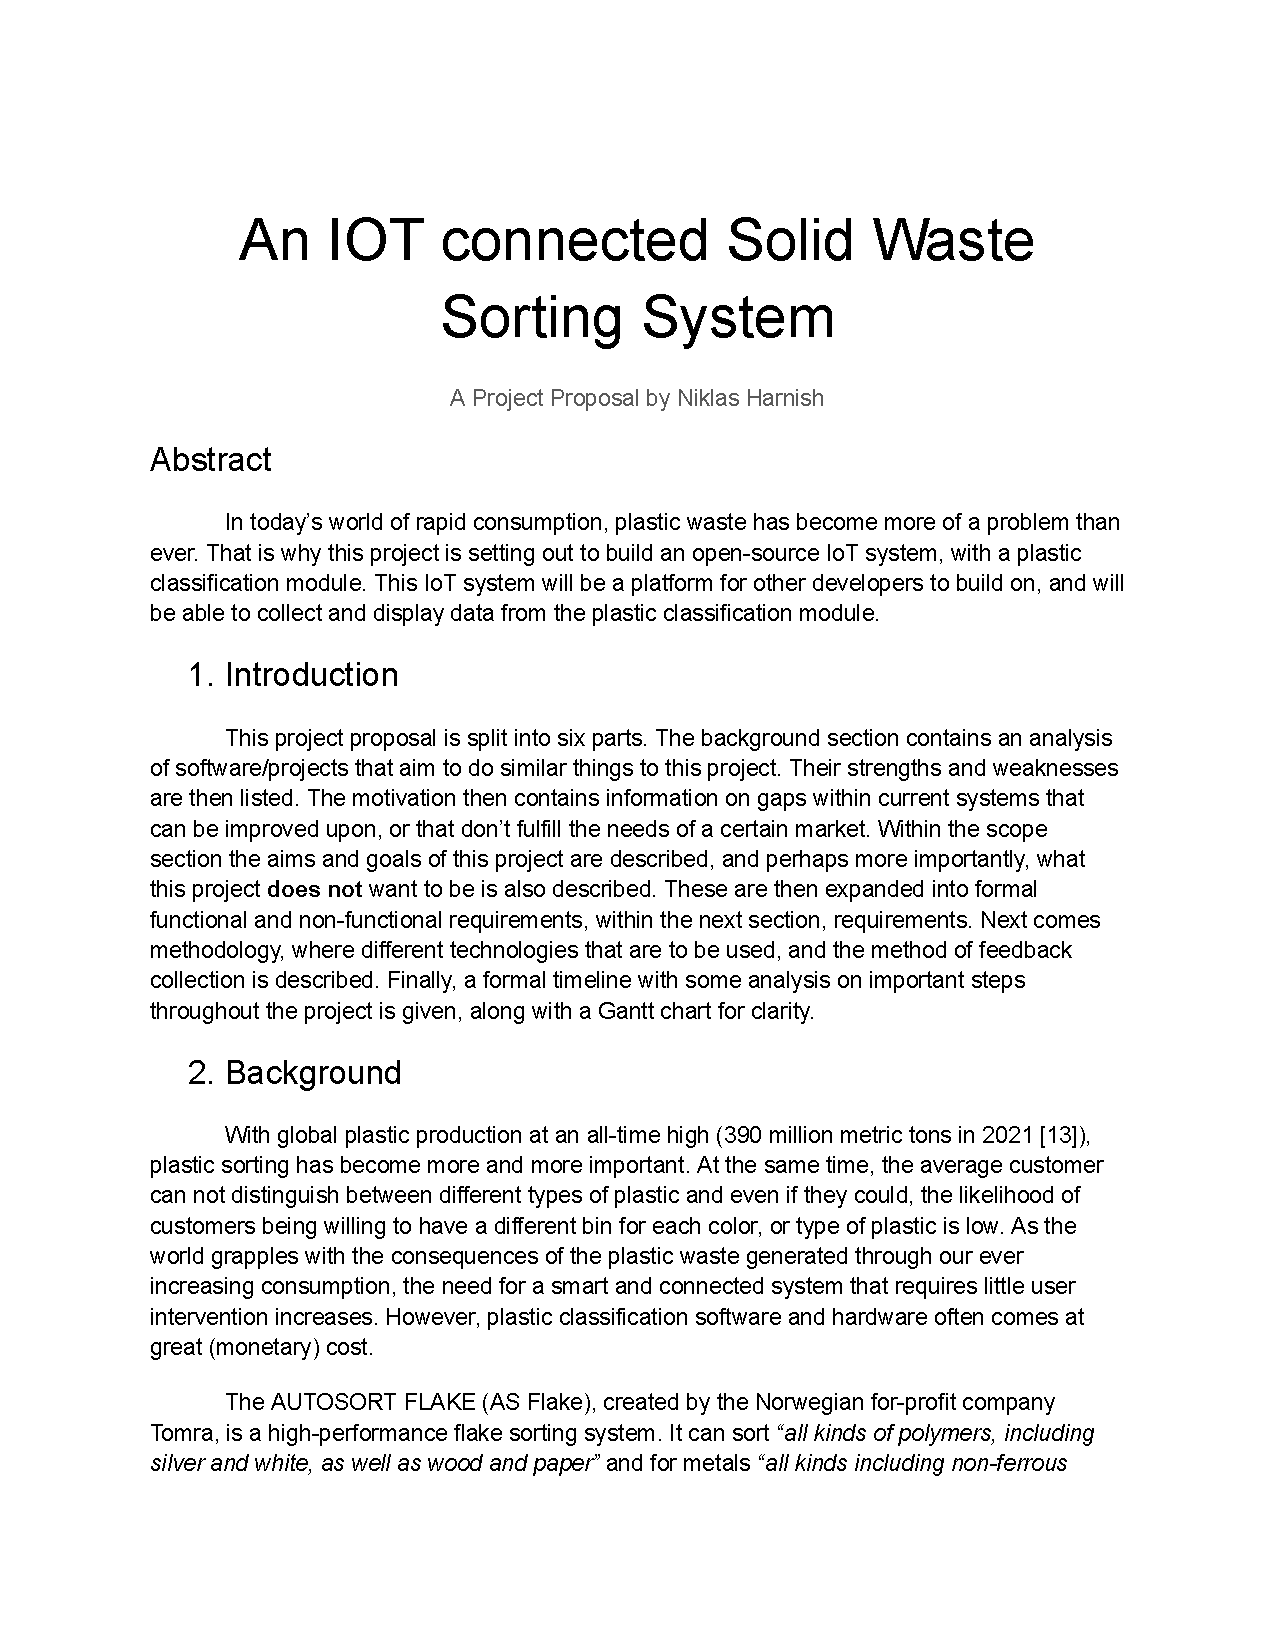
\includepdf[pages=-]{project_proposal.pdf}

\newpage

\chapter{Another Appendix Chapter}
\label{chap:A2}

This could be about your experiments

\end{document}
